\documentclass[a4paper,12pt,oneside,openany,table,xcdraw]{article}

\usepackage{setspace}
\usepackage{multirow}
\usepackage{hyperref}
\usepackage{caption}
\usepackage{indentfirst}

\usepackage[brazilian]{babel}
\usepackage[utf8x]{inputenc}
\usepackage{amsmath, graphicx, subfig, enumerate}
\usepackage{float, verbatim}
\usepackage[colorinlistoftodos]{todonotes}
\usepackage{makeidx} % Para o sumário
\usepackage{geometry}

\graphicspath{{img/}}
\geometry{a4paper, hmargin={3cm, 3cm}, vmargin={3cm, 2cm} }
\setlength{\parindent}{1.0cm}
\captionsetup{font=small}

\begin{document}
\newcommand{\thedepartment}{Faculdade de Engenharia Elétrica}
\newcommand{\thecourse}{FEELT}
\newcommand{\thetitle}{CIRCUITOS TRIFÁSICOS EQUILIBRADOS - MEDIDA DE POTÊNCIA COM 2 WATTÍMETROS }
\newcommand{\thetype}{Relatório da Disciplina de Experimental de Circuitos Elétricos II}
\newcommand{\theproftitle}{Bacharel em Engenharia Elétrica}
\newcommand{\thestudent}{Lesly Viviane Montúfar Berrios\\
\centering11811ETE001}
\newcommand{\theadvisor}{Prof. Wellington Maycon Santos Bernardes}
\newcommand{\thecity}{Uberlândia}

\thispagestyle{empty}\newcommand*{\themonth}{\ifthenelse{\the\month < 2}{Janeiro }
                  {\ifthenelse{\the\month < 3}{Fevereiro }
                  {\ifthenelse{\the\month < 4}{Março }
                  {\ifthenelse{\the\month < 5}{Abril }
                  {\ifthenelse{\the\month < 6}{Maio }
                  {\ifthenelse{\the\month < 7}{Junho }
                  {\ifthenelse{\the\month < 8}{Julho }
                  {\ifthenelse{\the\month < 9}{Agosto }
                  {\ifthenelse{\the\month < 10}{Setembro }
                  {\ifthenelse{\the\month < 11}{Outubro }
                  {\ifthenelse{\the\month < 12}{Novembro }{Dezembro }}}}}}}}}}}}
                  
\begin{titlepage}
\begin{center}

	\vspace{-0.5cm}

  \begin{figure}[hbt!]
		\begin{center}
		   
\includegraphics[width=2.8cm]{ufu-logo.png}
		\end{center}
	\end{figure}
 	%\vspace{-4cm}

%\begin{doublespacing}

  \Large{\textbf{Universidade Federal de Uberlândia}}\\
  \large{\thedepartment}\\
  \large{\thecourse}\\


\vspace{5.8cm}
  \par
  \large\textbf{\thetitle}
\vspace{5.8cm} 

%\end{doublespacing}
  \par
  \thetype\\
  por\\
  %\hspace{2cm}\large{}\\

\vspace{0.8cm}
\par
  \normalsize{\thestudent}\\ [2cm]
  \theadvisor

\par\vfill
  \thecity, \themonth / \the\year

\end{center}

\end{titlepage}

%% Comeca o documento !

\onehalfspacing
\tableofcontents % sumário
\newpage

\section{Objetivos} % 2,5%
 Verificar experimentalmente os conceitos teóricos sobre os métodos utilizados para medir a potência ativa trifásica das cargas. Além disso, comparar os resultados com os valores obtidos utilizando uma análise teórica. 

\section{Introdução teórica} % 5%
As primeiras linhas de transmissão de energia elétrica, que surgiram no final do século XIX, destinavam-se exclusivamente ao suprimento do sistema de iluminação, pequenos motores e sistema de tração (railway) e operavam em corrente contínua a baixa magnitude de tensão. A geração e transmissão usando os mesmos níveis de tensão das diferentes cargas restringiu a distância entre a planta de geração e os consumidores e a tensão da geração em corrente contínua não podia ser facilmente aumentada para a transmissão a grandes distâncias \cite{ph}. 

Para realizar uma transmissão de energia elétrica a grandes distâncias era necessário um nível elevado de magnitude de tensão, e essa tecnologia de conversão para corrente contínua não era viável naquela época. Por isso, foi necessária a mudança da transmissão de corrente continua para corrente alternada, devido principalmente aos seguintes motivos:

\begin{itemize}
\item O desenvolvimento e uso dos transformadores, permitindo a transmissão a grandes distâncias usando altos níveis de tensão, reduzindo as perdas elétricas dos sistemas e a queda de tensão.
\item A elevação/redução da magnitude de tensão é realizado com uma alta eficiência e a baixo custo através dos transformadores.
\item Surgimento de geradores e motores em corrente alternada, construtivamente mais simples, eficientes e baratos que as máquinas em corrente contínua
\end{itemize}

Assim, a corrente alternada seria a melhor alternativa para a transmissão de energia elétrica à grandes distâncias. Além disso, introduz-se o conceito de gerador trifásico, ilustrado pela Figura \ref{gerador}, no qual três bobinas defasadas em $120^\circ $ elétricos no espaço geram um conjunto de três tensões de mesmo valor máximo, defasadas de 120 graus elétricos no tempo.

Um gerador trifásico aproveita melhor o espaço físico, resultando em um gerador de tamanho reduzido e mais barato, comparado com os geradores monofásicos de igual potência, ademais são superiores aos motores monofásicos em rendimento, tamanho, fator de potência e capacidade de sobrecarga.
Um sistema monofásico precisa de dois condutores; e um sistema trifásico (perfeitamente balanceado) precisa de três condutores, porém conduz três vezes mais potência. Na prática, devido a pequenos desequilíbrios inevitáveis, os sistemas trifásicos contam com um quarto condutor, o neutro.

É possivel conectar as bobinas de gerador trifásicos em configuração estrela ou delta, assim como a carga em \emph{Conexão em estrela} (\ref{estrela}) ou  \emph{Conexão em delta/triângulo} (\ref{delta}).
\begin{figure}[H]
\centering
\captionsetup{font=scriptsize}
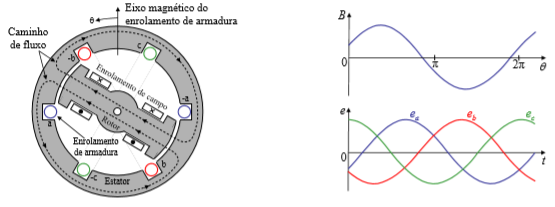
\includegraphics[width=14.5cm]{motor3phi}
\caption{Geração de tensão alternada trifásica.}
\label{gerador}
\end{figure}

\subsection{Carga em conexão em estrela} \label{estrela}
A carga na configuração estrela é caracterizada por ter uma tensão fase-neutro entre seus terminais e corrente de linha igual à corrente de fase ($I_L=I_F$). Ainda é possível determinar a tensão fase-fase ou de linha pela relação descrita na Figura \ref{carga-estrela} \cite{irwin}. 
\begin{figure}[H]
\centering
\captionsetup{font=scriptsize}
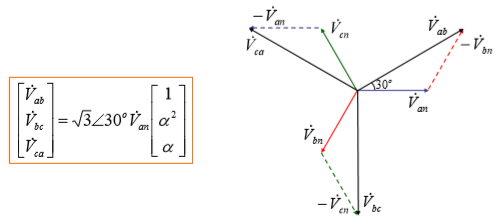
\includegraphics[width=14.5cm]{carga-estrela}
\caption{Relação entre tensão de linha e fase numa carga em estrela.}
\label{carga-estrela}
\end{figure}

\subsection{Carga em conexão em delta ou triângulo} \label{delta}
Já para a carga na configuração delta, ou triângulo, em seus terminais há uma tensão de linha igual a tensão de fase \cite{irwin}. Nesse caso, a relação entre linha e fase ocorre para a corrente, conforme descrito na Figura \ref{carga-delta}.
\begin{figure}[H]
\centering
\captionsetup{font=scriptsize}
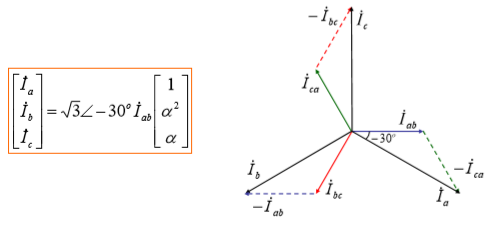
\includegraphics[width=14.5cm]{carga-delta}
\caption{Relação entre corrente de linha e fase numa carga em delta.}
\label{carga-delta}
\end{figure}

\subsection{Medição de potência pelo método dos 2 wattímetros} \label{potencias}
A medição de potência por meio de dois wattímetros analógicos possui o esquema de ligação mostrado na Figura \ref{watt:ligacao}.
\begin{figure}[H]
\centering
\captionsetup{font=scriptsize}
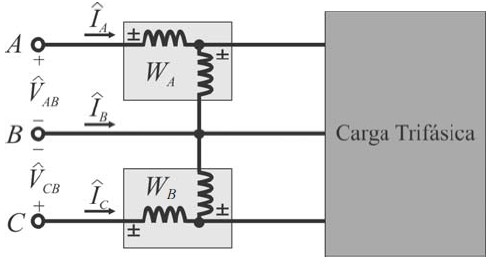
\includegraphics[width=13cm]{watt}
\caption{Esquema de ligação para medição de potência com 2 wattímetros.}
\label{watt:ligacao}
\end{figure}
Tem-se que para uma fase ABC, $W_A=W_2$ e $W_B=W_1$, uma vez que é usada a convenção das Equações (\ref{w1}) e (\ref{w2}).
\begin{gather}
W_1 = V_L \times I_L \times cos(\theta - 30^\circ)\label{w1}\\
W_2 = V_L \times I_L \times cos(\theta + 30^\circ)\label{w2}
\end{gather}
Assim, obtém-se as potências totais reativa e ativa, a partir da medição dos wattímetros, como observa-se em (\ref{PT}) e (\ref{QT}). Consequentemente é possível calcular outros parâmetros como defasagem tensão-corrente ou fator de potência, do que se percebe a facilidade desse método na prática.
\begin{gather}
P_{3\phi} = W_1 + W_2\label{PT}\\
Q_{3\phi} = \sqrt{3}(W_1 - W_2)\label{QT}
\end{gather}


\section{Preparação}
\subsection{Materiais e ferramentas} % 2,5%
\begin{enumerate}[1 -]
\item \emph{\textbf{Fonte:}}
Alimentará todo o circuito. Possui frequência de $60Hz$.

\item \emph{\textbf{Regulador de tensão (Varivolt):}}
Também chamado de autotransformador, permitirá obter o valor desejado de corrente a partir da regulagem correta da tensão fornecida pela fonte.

\item \emph{\textbf{Conectores:}}
Para as conexões no circuito foi utilizado majoritariamente cabos banana-banana.

\item \emph{\textbf{Medidor eletrônico KRON Mult K:}}
Possibilita encontrar a medição da potência real (P) - vatímetro, reativa (Q) e aparente (S) do circuito. Ele também possui função de cofasímetro, instrumento elétrico que mede o fator de potência (fp, $cos\theta$) ou o ângulo da impedância $\theta$ do circuito, para um circuito com a impedância $Z = Z\angle \theta$.

\item \emph{\textbf{Amperímetro analógico AC:}}
Instrumento utilizado para acompanhar visualmente o aumento da corrente.

\item \emph{\textbf{Reatores de 160 mH:}}
Foram utilizados 3, para compor a carga do circuito trifásico. Sendo $L=160mH$ e $R_L=3,8\Omega$. Pode haver pequena variação na indutância conforme a disponibilidade do dispositivo.

\item \emph{\textbf{Resistores de $50\Omega$:}}
Foram utilizados 3, para compor a carga do circuito trifásico.

\item \emph{\textbf{Capacitores de $45,9\mu F$:}}
Foram utilizados 3, para compor a carga do circuito trifásico. Sendo $C= 45,9\mu F$.

\end{enumerate}

\subsection{Montagem} % 2,5%

\subsubsection{Carga em estrela}
 Efetue a montagem indicada na Figura 1 abaixo, alimentando os pontos \textbf{a b c n} através de uma fonte alternada trifásica em seqüência de fases \textbf{abc} (ou \textbf{direta}), aplicando uma tensão entre linhas $V_L$ igual a $100 V$, em frequência de 60 Hz. Os parâmetros da carga são: $R = 50 \Omega$; $R_L = 3,8\Omega$; $L = 160 mH$. Na Figura \ref{fig1}, $V_L$ representa um voltímetro conectado para medir a tensão entre linhas; $A_L$ representa um amperímetro conectado para medir a corrente de linha (igual a de fase); $W_i$ representa um wattímetro analógico conectado para medir a potência ativa da carga. Os valores dos instrumentos devem ser anotados na Tabela \ref{tab1}.  

Utilize os medidores digitais \emph{Kron} para medida de corrente e tensão ($TL = 0048$ – $3\phi$ sem Neutro). Além disso, compare os valores das potências entre \emph{Kron} e os wattímetros analógicos. \textbf{Atente-se a escala do wattímetro (corrente e tensão)}. 
\begin{figure}[H]
\centering
\captionsetup{font=scriptsize}
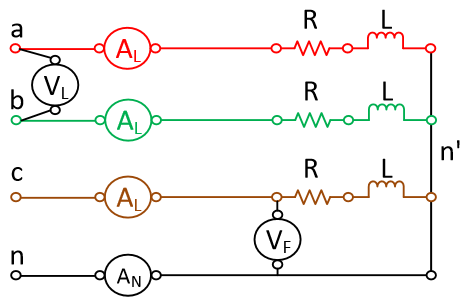
\includegraphics[width=14cm]{fig1}
\caption{Ligação em estrela em sequência de fases abc.}
\label{fig1}
\end{figure}
Observa-se pelo desenho que não é possível obter a tensão e corrente de todas as fases de forma simultânea, sendo necessária a mudança dos medidores $V_L$ e $V_F$ para a obtenção dos demais valores. Para isso, utilizaremos o medidor trifásico eletrônico \textit{Kron Mult-K} (wattímetro),  usando as entradas $V_A$, $V_B$, $V_C$, $V_N$ para as medidas de tensão e $I_A$, $I_B$ e $I_C$ para as medidas de corrente, assim sendo, realizando as ligações apropriadas. Como o \textit{Kron} não mede a corrente de neutro, então é necessário um amperímetro analógico $A_C$ entre $n$ e $n’$.

\begin{table}[H]\scriptsize
\centering
\def\arraystretch{1.35}
\captionsetup{font=scriptsize}
\captionof{table}{Ligação em triângulo em seqüência de fases abc.} \label{tab1}
\resizebox{\textwidth}{!}{ %
\begin{tabular}{|c|c|c|c|c|c|c|c|c|c|c|}
\hline
$V_{L} (V)$ & $I_{L} (A)$ & $W_{1} (W)$           & $W_{2} (W)$            & $P_{F} (W)$ & $P_{T} (W)$            & $Q_{F} (Var)$ & $Q_{T} (Var)$          & $S_{F} (VA)$ & $S_{T} (VA)$           & Fator de potência \\ \hline
99,46       & 0,501       & \multirow{3}{*}{5,00} & \multirow{3}{*}{50,00} & 16,15       & \multirow{3}{*}{51,44} & 25,01         & \multirow{3}{*}{75,43} & 29,60        & \multirow{3}{*}{90,96} & 0,543             \\ \cline{1-2} \cline{5-5} \cline{7-7} \cline{9-9} \cline{11-11} 
100,60      & 0,514       &                       &                        & 18,09       &                        & 24,52         &                        & 30,32        &                        & 0,596             \\ \cline{1-2} \cline{5-5} \cline{7-7} \cline{9-9} \cline{11-11} 
100,50      & 0,532       &                       &                        & 17,20       &                        & 25,90         &                        & 31,04        &                        & 0,556             \\ \hline
\end{tabular}%
}
\end{table}


Agora, troque duas fases na saída do \textit{varivolt} para obter a \textbf{sequência cba} da conexão acima. Anote os valores na Tabela \ref{tab2}.

\begin{table}[H]\scriptsize
\centering
\def\arraystretch{1.35}
\captionsetup{font=scriptsize}
\captionof{table}{Ligação em triângulo em seqüência de fases abc.} \label{tab2}
\resizebox{\textwidth}{!}{ %
\begin{tabular}{|c|c|c|c|c|c|c|c|c|c|c|}
\hline
$V_{L} (V)$ & $I_{L} (A)$ & $W_{1} (W)$            & $W_{2} (W)$           & $P_{F} (W)$ & $P_{T} (W)$            & $Q_{F} (Var)$ & $Q_{T} (Var)$          & $S_{F} (VA)$ & $S_{T} (VA)$           & Fator de potência \\ \hline
100,70      & 0,499       & \multirow{3}{*}{50,00} & \multirow{3}{*}{5,00} & 15,92       & \multirow{3}{*}{51,42} & 24,30         & \multirow{3}{*}{75,30} & 29,13        & \multirow{3}{*}{91,42} & 0,550             \\ \cline{1-2} \cline{5-5} \cline{7-7} \cline{9-9} \cline{11-11} 
100,50      & 0,540       &                        &                       & 17,17       &                        & 26,50         &                        & 31,68        &                        & 0,544             \\ \cline{1-2} \cline{5-5} \cline{7-7} \cline{9-9} \cline{11-11} 
100,90      & 0,523       &                        &                       & 18,33       &                        & 24,50         &                        & 30,61        &                        & 0,599             \\ \hline
\end{tabular}%
}
\end{table}


\subsubsection{Carga em triângulo}
Efetue a montagem indicada na Figura \ref{fig2} abaixo, alimentando os pontos \textbf{a b c}
através de uma fonte alternada trifásica em sequência de fases \textbf{abc} (ou \textit{direta}),
aplicando uma tensão entre linhas $V_L = 80 V$ (para que a corrente de linha não ultrapasse os $2\, A$), em frequência de 60 Hz. Os
parâmetros da carga são: $R = 50 \Omega$; $C = 45,9 \mu F$. Na Figura \ref{fig2}, $V_L$ representa um
voltímetro conectado para medir a tensão entre linhas; $A_F$ representa um amperímetro
conectado para medir a corrente de fase; $A_L$ representa o amperímetro conectado para
medir a corrente de linha; $W_i$ representa um wattímetro analógico conectado para medir
a potência ativa trifásica da carga. Os valores dos instrumentos devem ser anotados na
Tabela \ref{tab3}.

Utilize os medidores digitais Kron para medida de corrente e tensão ($TL = 0048$ – $3\phi$
sem Neutro). Além disso, compare os valores das potências entre \emph{Kron} e os
wattímetros analógicos. Atente-se a escala do wattímetro (corrente e tensão).
\begin{figure}[H]
\centering
\captionsetup{font=scriptsize}
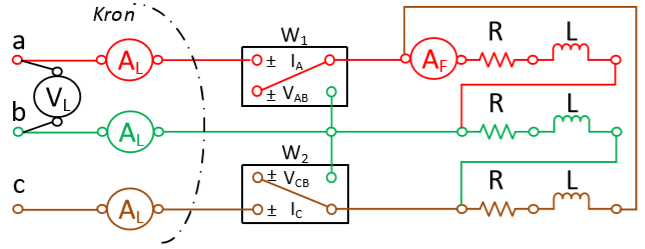
\includegraphics[width=14cm]{fig2}
\caption{Ligação em estrela em sequência de fases abc.}
\label{fig2}
\end{figure}

\begin{table}[H]\scriptsize
\centering
\def\arraystretch{1.35}
\captionsetup{font=scriptsize}
\captionof{table}{Ligação em triângulo em seqüência de fases abc.} \label{tab3}
\resizebox{\textwidth}{!}{ %
\begin{tabular}{|c|c|c|c|c|c|c|c|c|c|c|c|}
\hline
$V_{L} (V)$ & $I_{L} (A)$ & $I_{A_F} (A)$        & $W_{1} (W)$             & $W_{2} (W)$            & $P_{F} (W)$ & $P_{T} (W)$             & $Q_{F} (Var)$ & $Q_{T} (Var)$           & $S_{F} (VA)$ & $S_{T} (VA)$            & Fator de potência \\ \hline
79,53       & 1,782       & \multirow{3}{*}{0,5} & \multirow{3}{*}{132,50} & \multirow{3}{*}{25,00} & 55,44       & \multirow{3}{*}{164,68} & 61,57         & \multirow{3}{*}{185,39} & 81,65        & \multirow{3}{*}{245,23} & 0,673             \\ \cline{1-2} \cline{6-6} \cline{8-8} \cline{10-10} \cline{12-12} 
80,36       & 1,777       &                      &                         &                        & 54,24       &                         & 62,50         &                         & 81,76        &                         & 0,660             \\ \cline{1-2} \cline{6-6} \cline{8-8} \cline{10-10} \cline{12-12} 
80,59       & 1,787       &                      &                         &                        & 55,00       &                         & 61,32         &                         & 81,82        &                         & 0,667             \\ \hline
\end{tabular}%
}
\end{table}


Agora, troque duas fases na saída do \textit{varivolt} para obter a \textbf{sequência cba} da conexão acima. Anote os valores na Tabela \ref{tab4}.


\begin{table}[H]\scriptsize
\centering
\def\arraystretch{1.35}
\captionsetup{font=scriptsize}
\captionof{table}{Ligação em triângulo em seqüência de fases cba.} \label{tab4}
\resizebox{\textwidth}{!}{ %
\begin{tabular}{|c|c|c|c|c|c|c|c|c|c|c|c|}
\hline
$V_{L} (V)$ & $I_{L} (A)$ & $I_{A_F} (A)$        & $W_{1} (W)$            & $W_{2} (W)$             & $P_{F} (W)$ & $P_{T} (W)$             & $Q_{F} (Var)$ & $Q_{T} (Var)$           & $S_{F} (VA)$ & $S_{T} (VA)$            & Fator de potência \\ \hline
80,18       & 1,789       & \multirow{3}{*}{0,5} & \multirow{3}{*}{30,00} & \multirow{3}{*}{120,00} & 55,28       & \multirow{3}{*}{165,96} & 62,28         & \multirow{3}{*}{185,52} & 82,93        & \multirow{3}{*}{248,51} & 0,665             \\ \cline{1-2} \cline{6-6} \cline{8-8} \cline{10-10} \cline{12-12} 
80,45       & 1,776       &                      &                        &                         & 55,12       &                         & 61,55         &                         & 82,91        &                         & 0,667             \\ \cline{1-2} \cline{6-6} \cline{8-8} \cline{10-10} \cline{12-12} 
80,60       & 1,791       &                      &                        &                         & 55,56       &                         & 61,69         &                         & 82,67        &                         & 0,667             \\ \hline
\end{tabular}%
}
\end{table}

\section{Análise sobre segurança} % 2,5%
Os óculos de segurança são Equipamentos de Proteção Individual (EPIs) e são utilizados para a proteção da área ao redor dos olhos contra qualquer tipo de detrito estranho, que possa causar irritação ou ferimentos. Também protegem contra faíscas, respingos de produtos químicos, detritos, poeira, radiação e etc \cite{safe}.
É importante a utilização desse equipamento durante os experimentos a fim de evitar qualquer dano, além de preparar o profissional para o manejo correto e seguro de qualquer equipamento.
Além disso, foi de extrema importância a presença do professor ou técnico na verificação da montagem do circuito antes de energizá-lo. Assim, reduziu-se riscos de curtos-circuitos ou sobrecarga na rede.

\section{Análise teórica do circuito}
\subsection{Carga em estrela}
Correspondente à primeira montagem mostratada na Figura \ref{fig1} tem o circuito da Figura \ref{estrela:circuito}, o qual também será utilizado na simulação.
\begin{figure}[H]
\centering
\captionsetup{font=scriptsize}
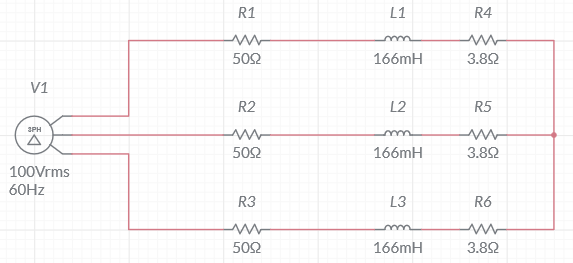
\includegraphics[width=13.5cm]{m1-esquema}
\caption{Circuito referente à montagem em estrela.}
\label{estrela:circuito}
\end{figure}
Do circuito esquemático Figura \ref{estrela:circuito}, considera-se primeiro sequência de fases positiva (abc), com $V_{AB}$ na referência tem-se os resultados mostrados a seguir.

\begin{gather*}
\begin{bmatrix}
V_{AB}\\
V_{BC}\\
V_{CA}
\end{bmatrix} =100V\ \begin{bmatrix}
1\\
\alpha ^{2}\\
\alpha 
\end{bmatrix}\\
V_{L} =V_{F}\sqrt{3} \ \angle 30^{\circ }\\
\begin{bmatrix}
V_{AN}\\
V_{BN}\\
V_{CN}
\end{bmatrix} =57,74V\ \angle -30^{\circ } \ \begin{bmatrix}
1\\
\alpha ^{2}\\
\alpha 
\end{bmatrix}\\
Z_{Y} =53,8+j\cdotp 1,04\ =82,53\angle 49,31^{\circ }\\
\theta _{Z} =49,31^{\circ }\\
fp=cos\ \theta _{Z} =cos\left( 49,31^{\circ }\right) =0,652\\
\\
W_{B} =W_{1} =100\cdotp 0,7\cdotp cos\left( 49,31^{\circ } -30^{\circ }\right) =66,06W\\
W_{A} =W_{2} =100\cdotp 0,7\cdotp cos\left( 49,31^{\circ } +30^{\circ }\right) =12,98W\\
P_{T} =W_{1} +W_{2} =66,06+12,98=79,04W\\
Q_{T} =\sqrt{3} \ ( W_{1} -W_{2}) =\sqrt{3} \ ( 66,06-12,98) =91,94 [VAr]\\
S_{T} =P_{T} +j\ Q_{T} =79,04+j\ 91,94=121,2\ \angle 49,31 [VA]\\
\end{gather*}

Para inversão de fase o cálculo é semelhante, havendo somente a permuta na medição de $W_A$ e $W_B$. Ademais, ccomo no experimento foi trocado somente a alimentação nas fases A e B, o wattímetro A continuou medindo $W_2$ de acordo com a convenção adotada, pois estará sobre a tensão $V_{CB}$. 
Abaixo, nas Tabelas \ref{comparacao corrente}, é visto um comparativo das informações obtidas.

\begin{table}[H]\scriptsize
\centering
\caption{Comparação das correntes na configuração estrela ABC.}
\label{m1:comp:IL}
\begin{tabular}{|c|c|c|c|}
\hline
Fases & \begin{tabular}[c]{@{}c@{}}$I_L$ (A)\\ experimental\end{tabular} & \begin{tabular}[c]{@{}c@{}}$I_L$ (A)\\ teórico\end{tabular} & Erro (\%) \\ \hline
A     & 0,501                                                            & \multirow{3}{*}{0,7}                                        & -28,43    \\ \cline{1-2} \cline{4-4} 
B     & 0,504                                                            &                                                             & -26,57    \\ \cline{1-2} \cline{4-4} 
C     & 0,532                                                            &                                                             & -24,00    \\ \hline
\end{tabular}
\end{table}

\begin{table}[H]
\centering
\caption{Comparativo de potências experimentais (\textbackslash{}emph\{Kron\}) e teórico, na configuração estrela ABC.}
\label{m1:comp:potencias}
\begin{tabular}{ccccc}
            & $P_{T}$ (W) & $Q_{T}$ (VAr) & $S_{T}$ (VA) & FP     \\
Experimento & 51,44       & 75,93         & 90,96        & 0,565  \\
Teórico     & 79,04       & 91,94         & 121,20       & 0,652  \\
Erro (\%)   & -34,92      & -17,41        & -24,95       & -13,34
\end{tabular}
\end{table}

Observe 


\subsection{Carga em delta}

\section{Cálculos, análise dos resultados e questões} % (quando houver) (70%)
\begin{enumerate}[1)]
\item Para os sistemas das Figuras 1 e 2, ao ser ligado, o que aconteceu com os wattímetros $W_1$ e $W_2$ quando a sequência de fases foi invertida? Algum deles marcou valor negativo? Explique. Encontre as potências usando as leituras. 

\vspace{0.8mm}
\textbf{Resposta.} Quando  a sequência de fases foi invertida, houve uma permuta entre as leituras dos wattímetros $W_1$ e $W_2$, uma vez que o sistema é equilibrado, e, no caso deste experimento em especial, não foi marcado nenhum valor negativo. Daria negativo no caso em que o fator de potência $cos \theta <0,5$, conforme mostrado na Figura \ref{fp}.
\begin{figure}[H]
\centering
\captionsetup{font=scriptsize}
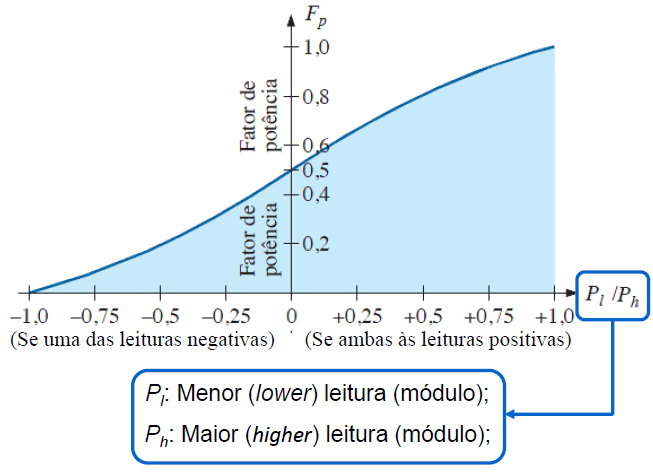
\includegraphics[width=13cm]{fp}
\caption{Curva das Relações de Potência no Método dos Dois Wattímetros \cite{ph}.}
\label{fp}
\end{figure}

Para o cálculo das potências utilizando-se as leituras dos wattímetros tem-se a teoria descrita na seção \ref{potencias}. Assim, para a sequência , $P_{3\phi}=W_1+W_2 = 5,00 + 50,00 = 55 W$ e $Q_{3\phi} = \sqrt{3}\ (W_1 - W_2) = \sqrt{3}\ (50 - 5) = 77,94 VAr$ e como a potência aparente é dada por $S=P+Qj$, tem-se $S= 55 + 77,94\cdot j \Rightarrow S_{3\phi} = 95,392\angle 54,79$ [VA]. O resultado visual teórico e experimental é visto na Figura \ref{pot-tab1}. Note que o triângulo de potências é o mesmo para ambas as sequências, uma vez que a permuta das leitura nos wattímetros também permuta os valores a serem considerados como $W_1$ e $W_2$ (que agora será o wattímetro conectado a tensão $V_{CB}$). %%%%%%%%%%%%%%%%%%%%%%%%%%%%%%%%%%%%%%%%%%%%%%%%%%%%%%%%%%%%%%%%%%%%%%%%%%%%%%%% usei a convencao usada nas aulas do Paulo H

\begin{figure}[H]
\centering
\captionsetup{font=scriptsize}
\subfloat[]{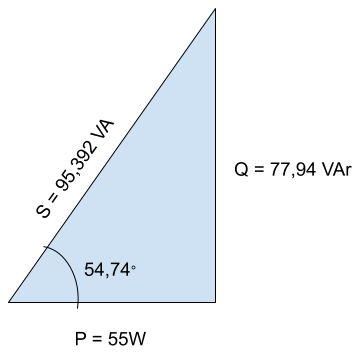
\includegraphics[width=0.33\textwidth]{pot-teorico1}}\hfill
\subfloat[]{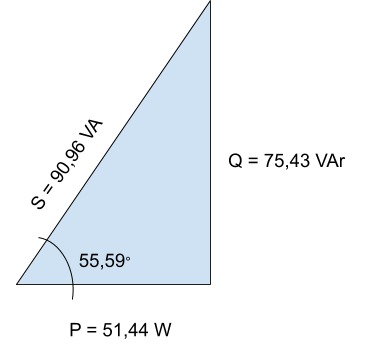
\includegraphics[width=0.33\textwidth]{pot-exp1}}\hfill
\subfloat[]{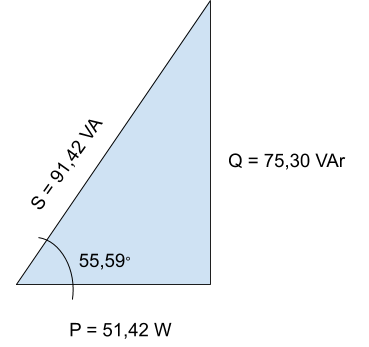
\includegraphics[width=0.33\textwidth]{pot-exp2}}
\caption{Comparação das potências obtidas no caso estrela (a) teórico, (b) \textbf{abc} experimental, (c) \textbf{cba} experimental.}
\label{pot-tab1}
\end{figure}


\item  Encontre o valor das leituras dos wattímetros usando as expressões analíticas. \vspace{0.8mm}

\textbf{Resposta.} A leitura dos wattímetros dos wattímetros $W_1$ e $W_2$ analiticamente são descritas pelas Equações (\ref{w1}) e (\ref{w2}), conforme na Seção \ref{potencias}.
\begin{gather}
W_1 = V_L \times I_L \times cos(\theta - 30^\circ)\label{w1}\\
W_2 = V_L \times I_L \times cos(\theta + 30^\circ)\label{w2}
\end{gather}

Assim, analiticamente tem-se os resultados da Tabela \ref{w}.

\begin{table}[H]\scriptsize
\centering
\def\arraystretch{1.35}
\captionsetup{font=scriptsize}
\caption{Cálculo de $W_1$ e $W_2$ analiticamente.}
\resizebox{\textwidth}{!}{%
\begin{tabular}{cc|c|c|c|c|c|c|c|c|}
\cline{3-10}
                                               &                & $V_{L} (V)$ & $I_{L} (A)$ & $cos \theta$ & $\theta\, (^\circ)$ & $cos (\theta - 30^\circ)$ & $cos (\theta + 30^\circ)$ & $W_{1} (W)$ & $W_{2} (W)$ \\ \hline
\multicolumn{1}{|c|}{\multirow{2}{*}{Estrela}} & ABC ($V_{AB}$) & 99,46       & 0,501       & 0,543        & 57,11               & 0,890                     & 0,050                     & 44,35       & 2,51        \\ \cline{2-10} 
\multicolumn{1}{|c|}{}                         & CBA ($V_{CB}$) & 100,70      & 0,499       & 0,550        & 56,63               & 0,894                     & 0,059                     & 44,92       & 2,95        \\ \hline
\multicolumn{1}{|c|}{\multirow{2}{*}{Delta}}   & ABC            & 79,53       & 1,782       & 0,673        & 47,70               & 0,953                     & 0,213                     & 135,06      & 30,19       \\ \cline{2-10} 
\multicolumn{1}{|c|}{}                         & CBA            & 80,18       & 1,789       & 0,665        & 48.32               & 0,949                     & 0,202                     & 136,13      & 28,98       \\ \hline
\end{tabular}%
}
\label{w}
\end{table}

\item  Mostre através de um diagrama fasorial que de acordo com as polaridades das bobinas de corrente e de potencial a leitura do wattímetro analógico é positiva para um ângulo $| \theta_Z| < 60^\circ$. Mostre que a leitura será negativa se $| \theta_Z| > 60^\circ$. \vspace{0.8mm}

\textbf{Resposta.} 

\item  Mostre através de um diagrama fasorial que se a polaridade de uma das bobinas não for seguida a leitura terá um sinal oposto ao correto.  \vspace{0.8mm}

\textbf{Resposta.} 


\end{enumerate}

\newpage
\section{Simulação computacional} % (10%);
\subsection{Carga em conexão estrela}
\begin{figure}[H]
\centering
\captionsetup{font=scriptsize}
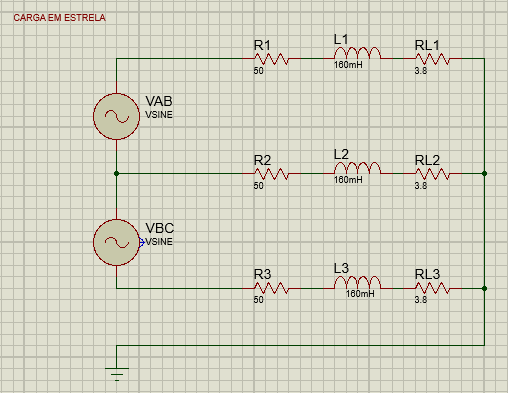
\includegraphics[width=14cm]{sim1}
\caption{Circuito da carga em conexão estrela.}
\label{sim1}
\end{figure}

\begin{figure}[H]
\centering
\captionsetup{font=scriptsize}
\subfloat[]{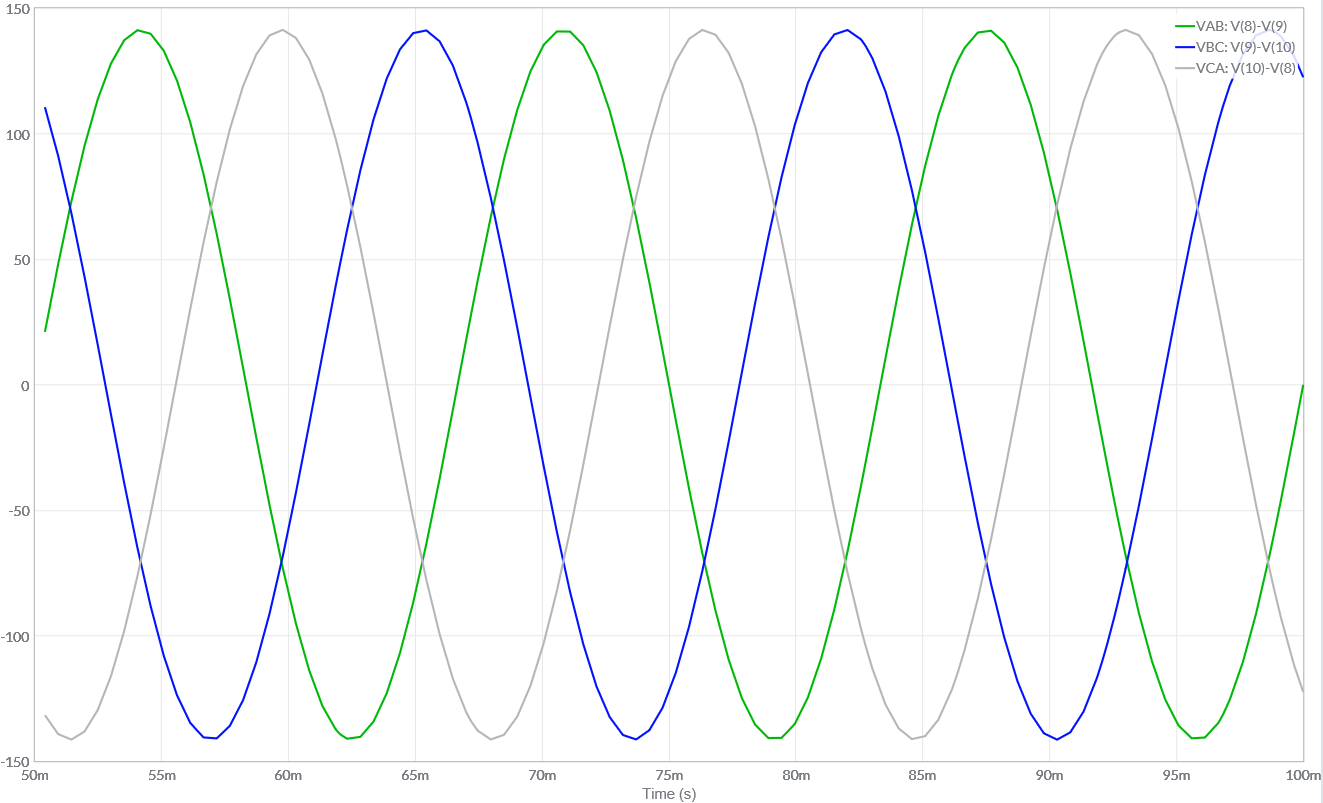
\includegraphics[width=0.8\textwidth]{m1-tensao}}

\subfloat[]{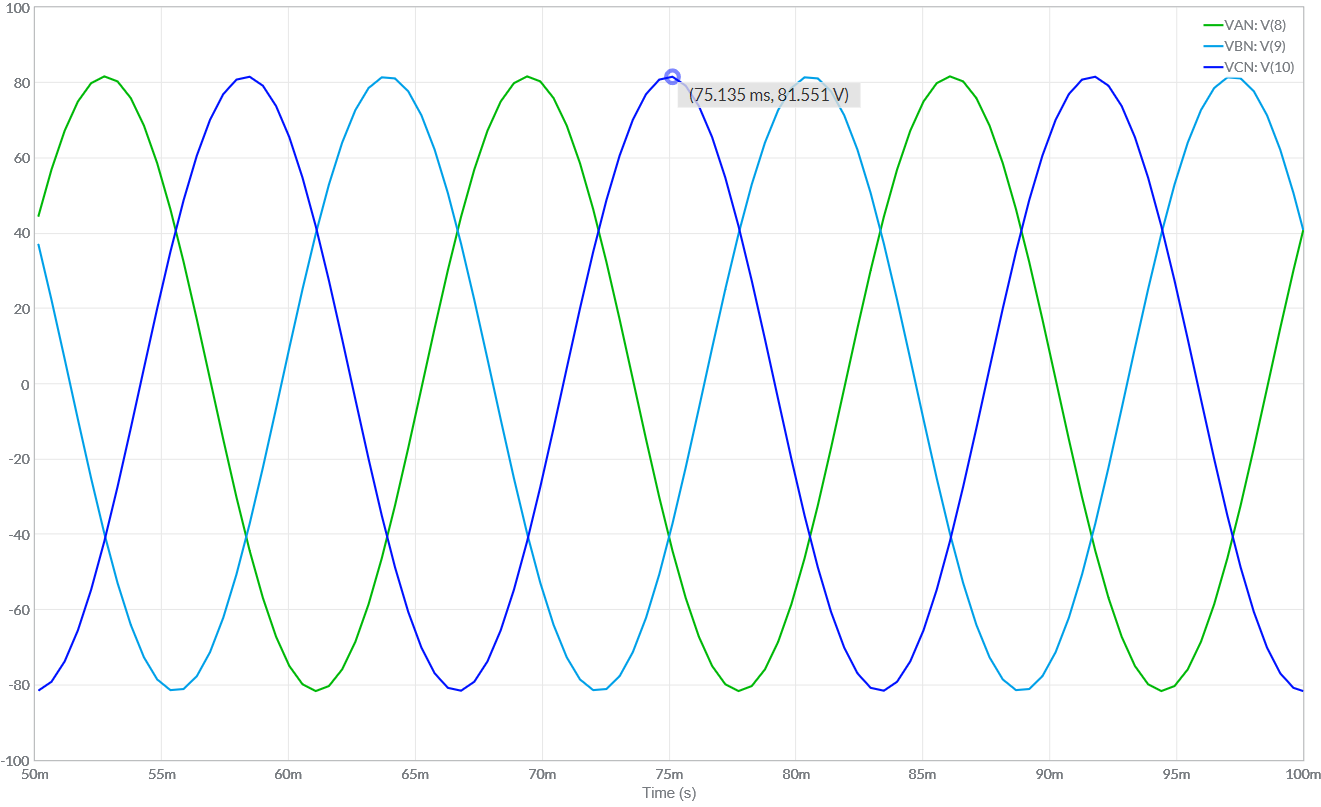
\includegraphics[width=0.8\textwidth]{m1-tensao-fase}}

\subfloat[]{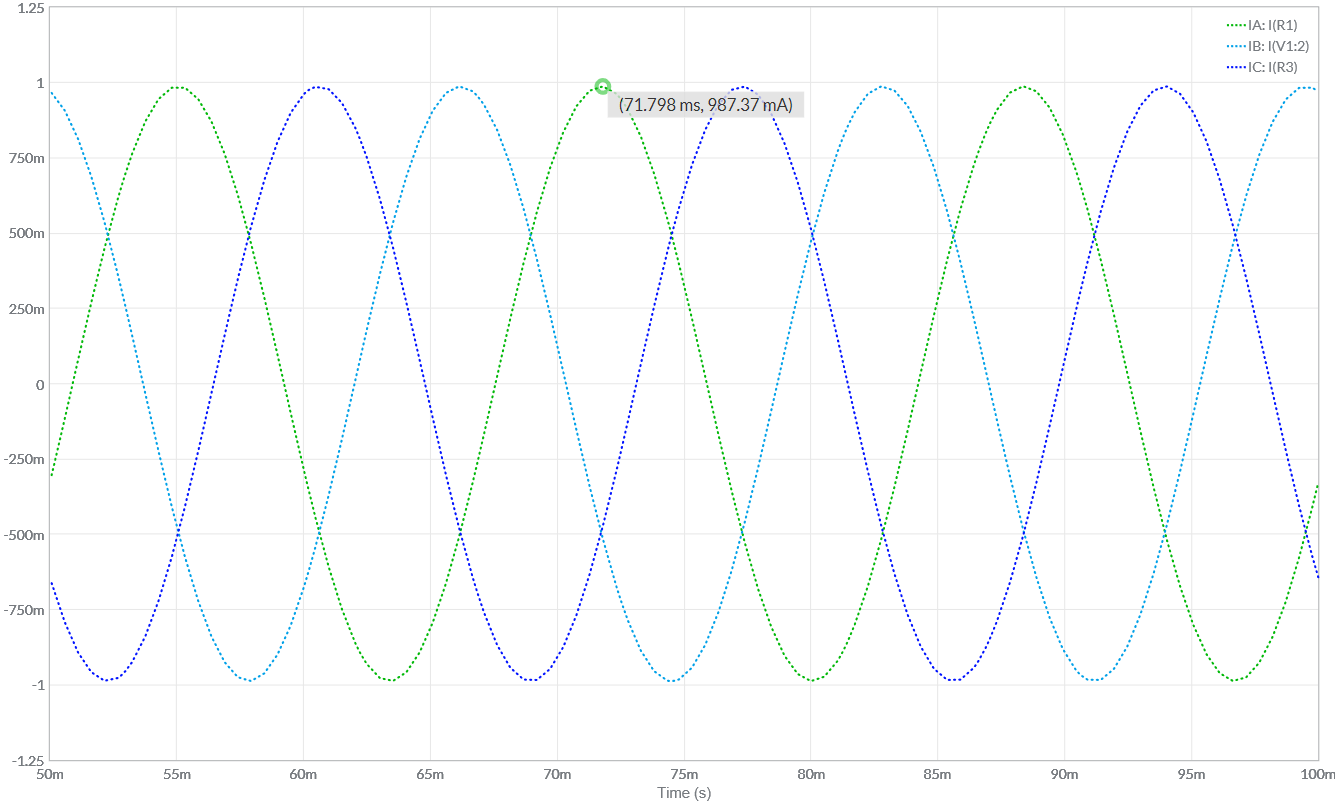
\includegraphics[width=0.8\textwidth]{m1-correntes}}
\caption{Comparação das potências obtidas no caso estrela (a) teórico, (b) \textbf{abc} experimental, (c) \textbf{cba} experimental.}
\label{pot-tab1}
\end{figure}


\subsection{Carga em conexão delta}
\begin{figure}[H]
\centering
\captionsetup{font=scriptsize}
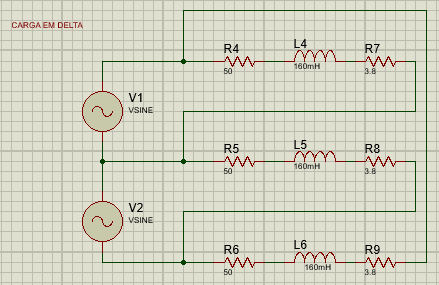
\includegraphics[width=14cm]{sim2}
\caption{Circuito da carga em conexão delta.}
\label{sim2}
\end{figure}

\section{Conclusões} % (no mínimo 10 linhas) (5%);
Neste experimento investiga-se as acerca de circuitos trifásicos equilibrados e suas particularidades em configuração delta e estrela. A análise experimental permitiu confirmar relações teóricas como $V_L=V_F\cdot\sqrt{3}$ para uma carga em estrela e $I_L = \sqrt{3}\cdot I_F$ para uma carga em delta. Além de verificar que para ambas configurações as potências (real e reativa) são as mesmas, devido as às duas relações teóricas já mencionadas apresentarem certa simetria.

Outro ponto importante verificado neste experimento é a inexistência de corrente no neutro para um circuito equilibrado. Assim, não é correto conferir corrente de curto-circuito pela corrente no neutro, já que idelamente tem valor nulo. As principais causas para a existência de corrente no neutro são: circuito em desequilíbrio, ou seja, as cargas possuem distintos valores de impedância e a LKC indica que haverá corrente no neutro; mal contato numa das fases ou rompimento dos conectores, nesse caso aparece corrente no neutro que será a soma fasorial das correntes nas fases que restaram, logo de módulo $I_F$, pois estão defasadas de $120^\circ$.  

\newpage
\begin{thebibliography}{9} 
% Introdução
\bibitem{ph}
    P. H. O. Rezende,
    "Circuitos Polifásicos Equilibrados", 2018.

\bibitem{irwin}
    J. D. Irwin,
    “Análise de Circuitos Em Engenharia”, Pearson, $4^a$ Ed., 2000.

\bibitem{boylestad}
    R. L. Boylestad,
    “Introdução À Análise de Circuitos”, Pearson, $10^a$ Ed., 2004.

\bibitem{safe}
    SafetyTrabi,
    “Óculos de segurança: Saiba quando utilizar este EPI”, SafetyTrab, 2019.
 Disponível em:
 \url{https://www.safetytrab.com.br/blog/oculos-de-seguranca/}. Acesso em: ago. 2019.


\end{thebibliography}
\end{document}
